\documentclass{standalone}
\usepackage{tikz}
\usepackage{amsmath}

\usetikzlibrary{arrows.meta,decorations.pathreplacing}

\tikzset{
    line/.style={
        thick
    },
    arrow/.style={
        line,
        ->,
        > = {
            Triangle[length=2.0mm, width=2.0mm]
        }
    }
}

% Switch to Sans Serif font.
\renewcommand{\familydefault}{\sfdefault}

\renewcommand{\wedge}{$\vphantom{\big|}$}


\begin{document}
\begin{tikzpicture}[xscale=1]
    \node (data1) at (0, 0) {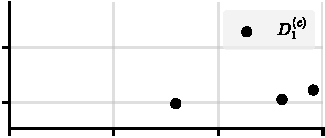
\includegraphics[height=1.5cm]{nps/datas_and_predictions/data1.pdf}};
    \node [right=2cm of data1] (pred1) {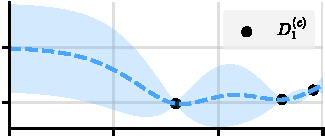
\includegraphics[height=1.5cm]{nps/datas_and_predictions/pred1.pdf}};
    \node [right=2cm of data1] (pred1) {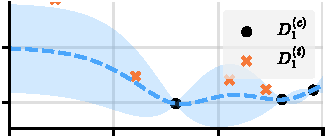
\includegraphics[height=1.5cm]{nps/datas_and_predictions/test1.pdf}};
    \node [yshift=5pt] () at ($(data1)!0.5!(pred1)$) {\LARGE $\overset{\phi}{\mapsto}$};
    %
    \node [above=0.2cm of data1] (datas) {\strut data sets $\mathcal{D}$};
    \node [above=0.2cm of pred1] (preds) {\strut predictions $\mathcal{P}$};
    \node at ($(datas)!0.5!(preds)$) {\LARGE $\to$};
    \node [left=0.1cm of datas, yshift=1pt] {\LARGE $\phi\colon$};
    %
    \node [below=-0.15cm of data1] () {\LARGE $\vdots$};
    \node [below=-0.15cm of pred1] () {\LARGE $\vdots$};
    %
    \node [below=0.75cm of data1] (data2) {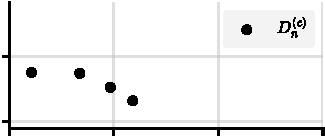
\includegraphics[height=1.5cm]{nps/datas_and_predictions/data2.pdf}};
    \node [right=2cm of data2] (pred2) {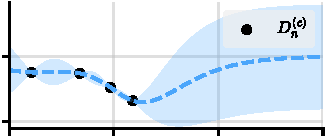
\includegraphics[height=1.5cm]{nps/datas_and_predictions/pred2.pdf}};
    \node [right=2cm of data2] (pred2) {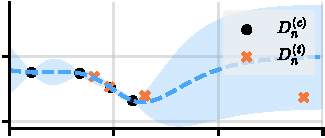
\includegraphics[height=1.5cm]{nps/datas_and_predictions/test2.pdf}};
    \node [yshift=5pt] () at ($(data2)!0.5!(pred2)$) {\LARGE $\overset{\phi}{\mapsto}$};
    %
    % \draw [arrow, <-] ($(data2)!0.5!(pred2) + (0, 0.6cm)$)  -- node [pos=1, anchor=south] {neural process} ++(0, 0.4cm);
    %
    \draw [dashed, thick] (-3, -3.75)
        --
            node [pos=0, anchor=north west, rotate=90, xshift=40pt] {meta-training}
            node [pos=0, anchor=north east, rotate=90, xshift=-5pt] {meta-testing}
        (8.8, -3.75);
    %
    \node [below=0.75cm of data2] (data3) {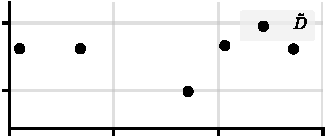
\includegraphics[height=1.5cm]{nps/datas_and_predictions/data3.pdf}};
    \node [right=2cm of data3] (pred3) {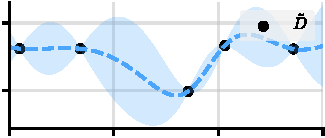
\includegraphics[height=1.5cm]{nps/datas_and_predictions/pred3.pdf}};
    \node [yshift=5pt] () at ($(data3)!0.5!(pred3)$) {\LARGE $\overset{\phi}{\mapsto}$};
\end{tikzpicture}
\end{document}